%Intro_El_Measurment
Last week we tackled very simple computer control, but we said we also want
to transfer data from our experiment to our computer. In order to understand
how to do that, we need to know what things we can measure with electronic
devices. We will take on this question today, but we will get practice
making these measurements with special equipment designed just for making
these measurements. These devices won't send the data they measure to our
computers, but they will display it so we can see the data.

Once we know how to make some basic measurements with these stand-alone
instruments, then we can consider how we would make a new instrument to
measure something else. We will build a current measuring device, an \emph{%
ammeter} out of electrical components and a \emph{voltmeter}. This will be
something we do over and over again. We will build a new instrument using
instruments we already know and some electrical equipment.

This lab consists of a large pre-reading section that will give you
background information, and then at the end an assignment where I\ will ask
you to practice making these measurements with our equipment. Notice this is
different than last week's lab reading. Last week the reading went step by
step through the assignment. This week the assignment is at the end and you
will have to think through how to do the problems as a group.

\section{What we measure: Voltage (and Current)\label{Voltage Measurement
with Meter}}

The two easiest electrical measurements to make are voltage and current
measurements. So physicists try to turn all other types of measurements into
voltage or current measurements. You may want to measure relative humidity.
But to record relative humidity on our computer we need to convert relative
humidity into a voltage or current! We will do experiments that do this type
of conversion, but first, let's learn about voltage and current so we can
see how electronic systems measure them.

Voltage is really \textquotedblleft electrical potential
difference,\textquotedblright\ which is the difference between electrical
potential energy per unit charge at two different circuit locations. Last
lab we said voltage was a comparison, and this is the comparison. We compare
the potential energy at two different circuit locations, only we divide the
potential energy by the charge of an electron.

To get a feel for how this works, think of a change in gravitational
potential energy, $\Delta U_{g}$. If we wanted to measure the difference in
potential energy between the top of a hill and the bottom of a hill, we
would need to place some sort of device both at the top and at the bottom of
the hill. \begin{figure}[h!]
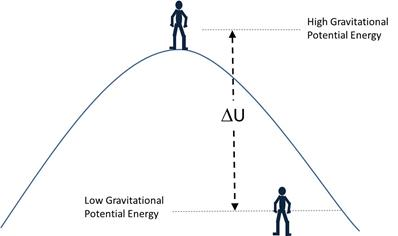
\includegraphics[width=3.3537in,height=1.9977in]{PH4CAU0F}
\end{figure}We have to do the same thing in
our electrical case. We need two \textquotedblleft
probes,\textquotedblright\ one placed at the high potential and one placed
at the low potential. For example, we could have the circuit that you see in
the next figure.\begin{figure}[h!]
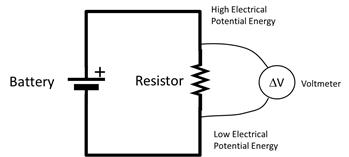
\includegraphics[width=2.9438in,height=1.3353in]{PH4CAU0G}
\end{figure}The positive end of the battery
is like the top of the hill. It provides a high electrical potential energy.
So we put one probe at the top of the \textquotedblleft
hill\textquotedblright\ or the plus side of the battery, and the other on
the bottom of the \textquotedblleft hill\textquotedblright\ or minus side of
the battery. The negative side of the battery provides a low electrical
potential energy. \emph{\ }With this we measure how high our potential
\textquotedblleft hill\textquotedblright\ is. The difference between these
two measurements is called \emph{voltage. }You should ask yourself
\textquotedblleft what would happen if you got the probes
backward?\textquotedblright\ 

In the next figure you can see how to actually perform this voltage
measurement with one of our meters.\begin{figure}[h!]
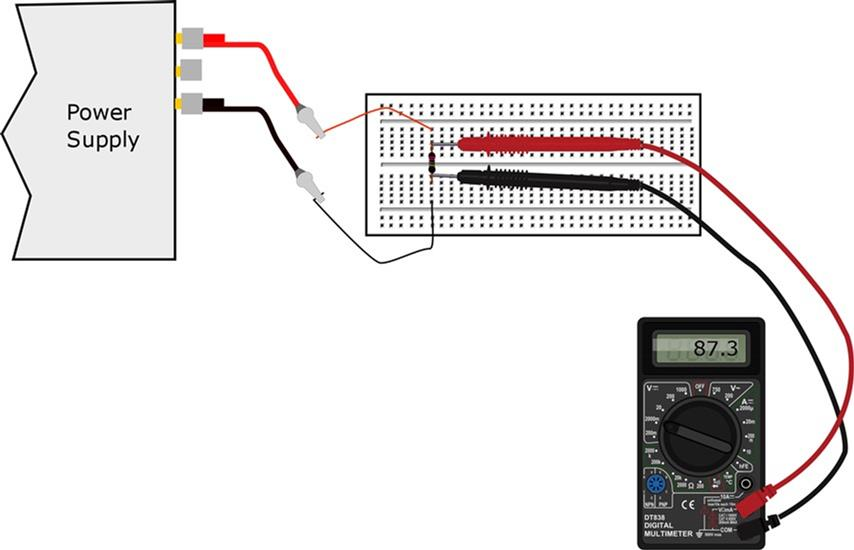
\includegraphics[width=5.5997in,height=3.614in]{PH4CAU0H}
\end{figure}

We say we measure voltage \textquotedblleft across\textquotedblright\ a
circuit element. This makes some sense if you consider that we very seldom
stand batteries up so their electric potential is greater in the same
direction as their gravitational potential. Batteries, resisters,
capacitors, etc., often lie down, and we measure \textquotedblleft
across\textquotedblright\ them by putting the positive probe on the high
potential side and the negative probe on the low potential side. Even though
the battery is lying down, we are still measuring a higher and lower
potential energy difference. Knowing a little about voltage, let's look at
our devices that produce voltages and then the devices that measure voltages.

\section{Experimental Hardware}

In today's lab we will study different hardware devices. A multimeter, power supply, a signal generator, and an oscilloscope. We will call these \textquotedblleft stand alone\textquotedblright\ instruments because they are independent boxes that do their job of measuring or generating signals without a computer connected to them. We will also look at the Arduino and how it can perform many of the same functions as the stand alone instruments. The power supply and the signal generator make voltage signals. The other devices measure them. Most of these devices are not to expensive to require students to purchase for just one lab. For this reason as a remote lab we will not be able to use them directly. You will likely encounter something like them at some point in your career so I've still included sections here for you to read. 

The Arduino acts as both a voltmeter and a power supply. It to can act as a stand alone instrument, but can also be used with a computer. For the first part of the class we will keep it connected to a computer to both tell it what to do and to read what it is measuring. Later labs we will explore using it without a computer. In this lab we will briefly explore how it can be used as a power supply and as a voltmeter in section \ref{ArduinoTour}. 

\subsection{Voltmeter/Multimeter}

Our first measurement device is voltmeter. It measures the electric potential (voltage) between its two leads (sometimes called \textquotedblleft probes\textquotedblright ). Here is a picture of one of our multi-meters set to measure voltage.

\begin{figure}[h!]
	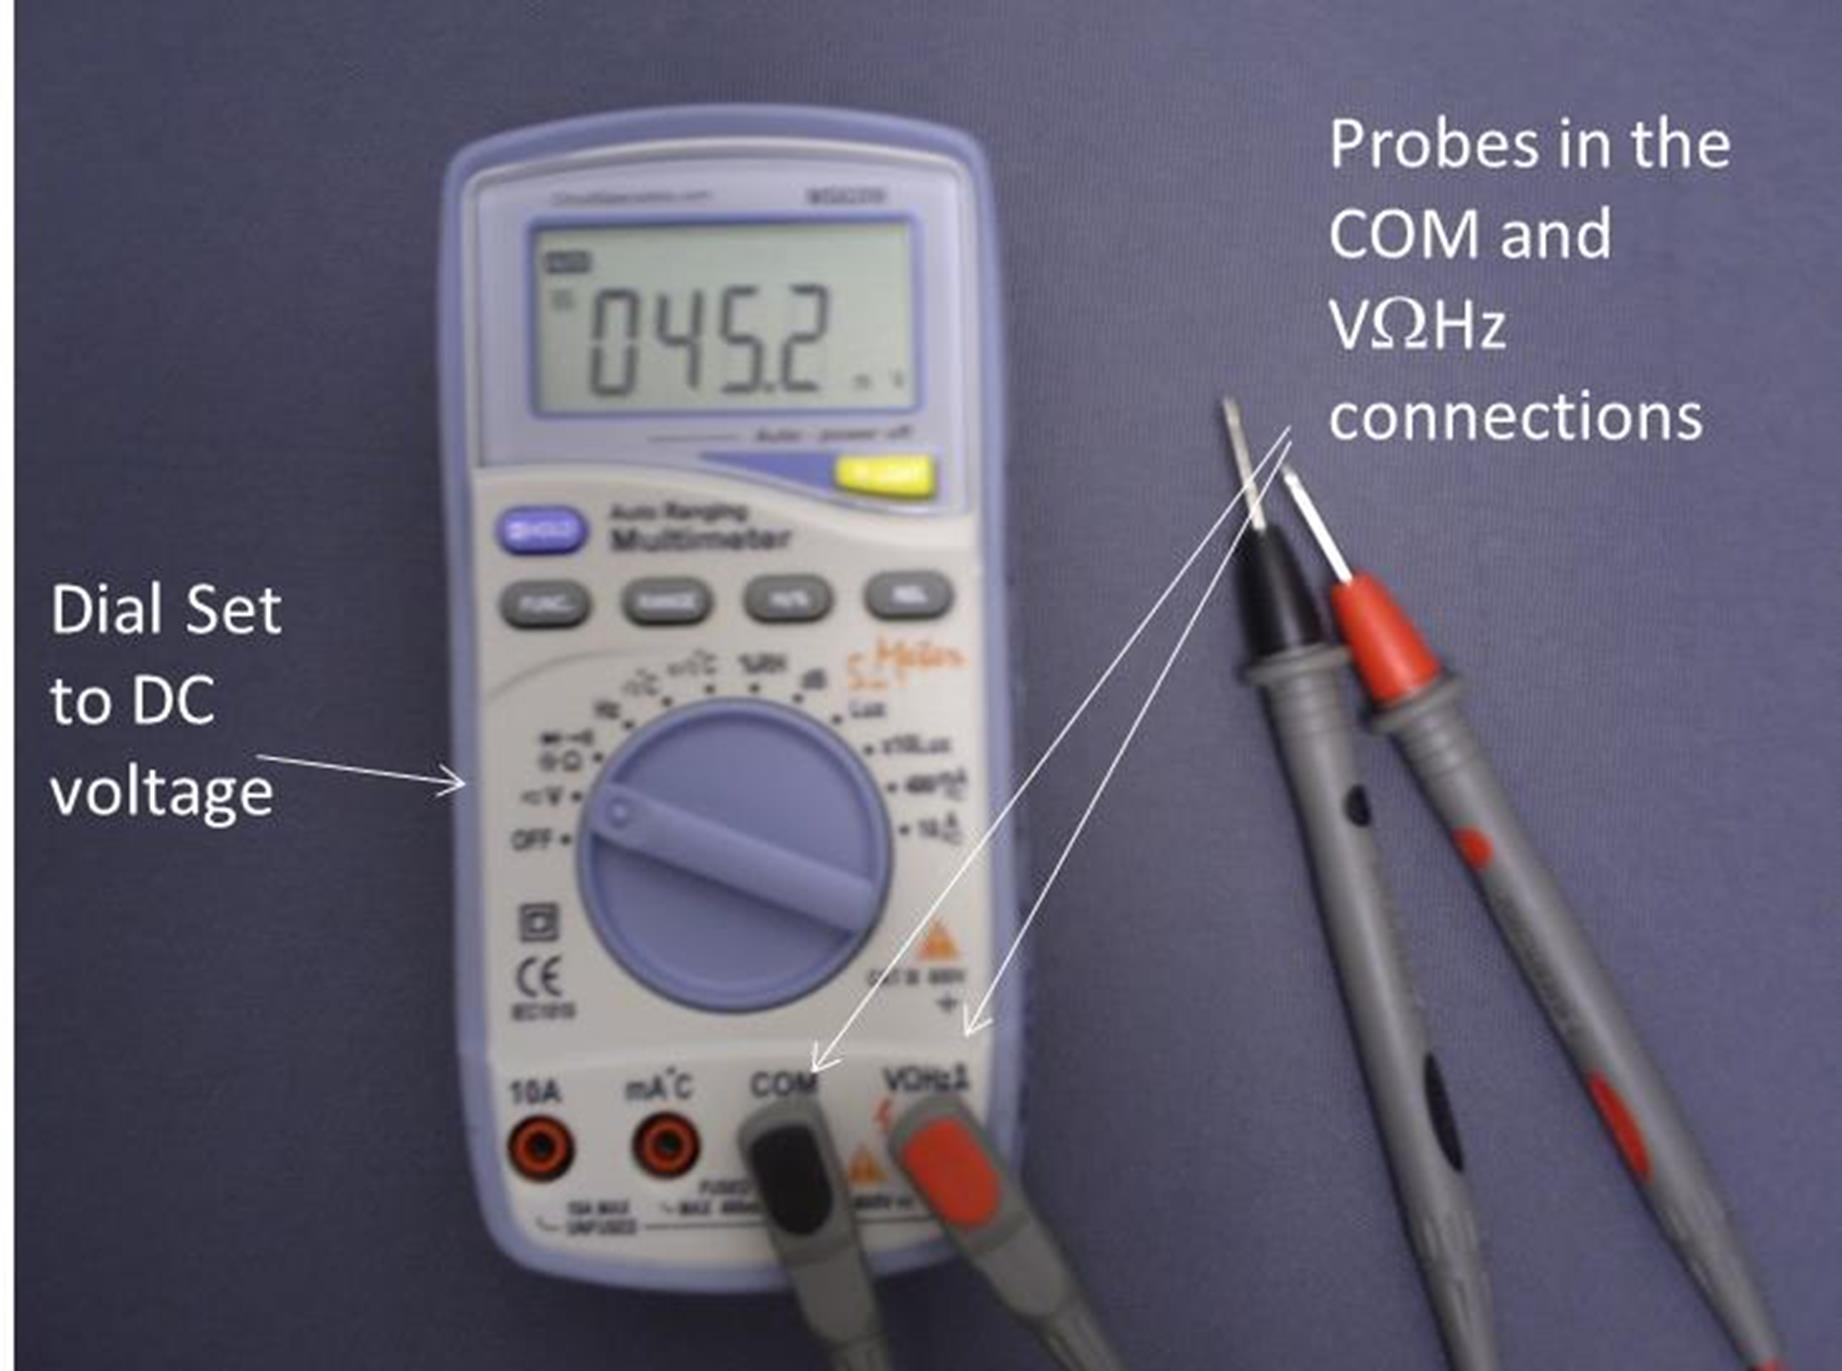
\includegraphics[width=3.116in,height=2.3266in]{PH4CAU0L}
\end{figure}

The display is set to read voltage by turning the dial to the $\unit{V}$ position. There are often two voltage settings. The one that has a wavy line next to it is alternating voltage. The one that has a straight line with three dots under it is the direct current (DC) voltage. These words might not mean much to you yet because you are just starting PH220. So for now, we will just use the DC voltage setting. As you learn more, we may use the alternating voltage setting. The leads (probes) should be connected to the COM (common) and $\unit{V}\unit{\Omega}\unit{Hz}$ connectors. Note that connecting your probe leads to the wrong position can blow the fuse (or worse) in your meter and make subsequent readings very wrong. You should make sure you don't do this, and watch to make sure someone else has not done this before you. If the meter seems crazy, it just may be. We have several different voltmeter models. Here is a picture of a different model.

\begin{figure}[h!]
	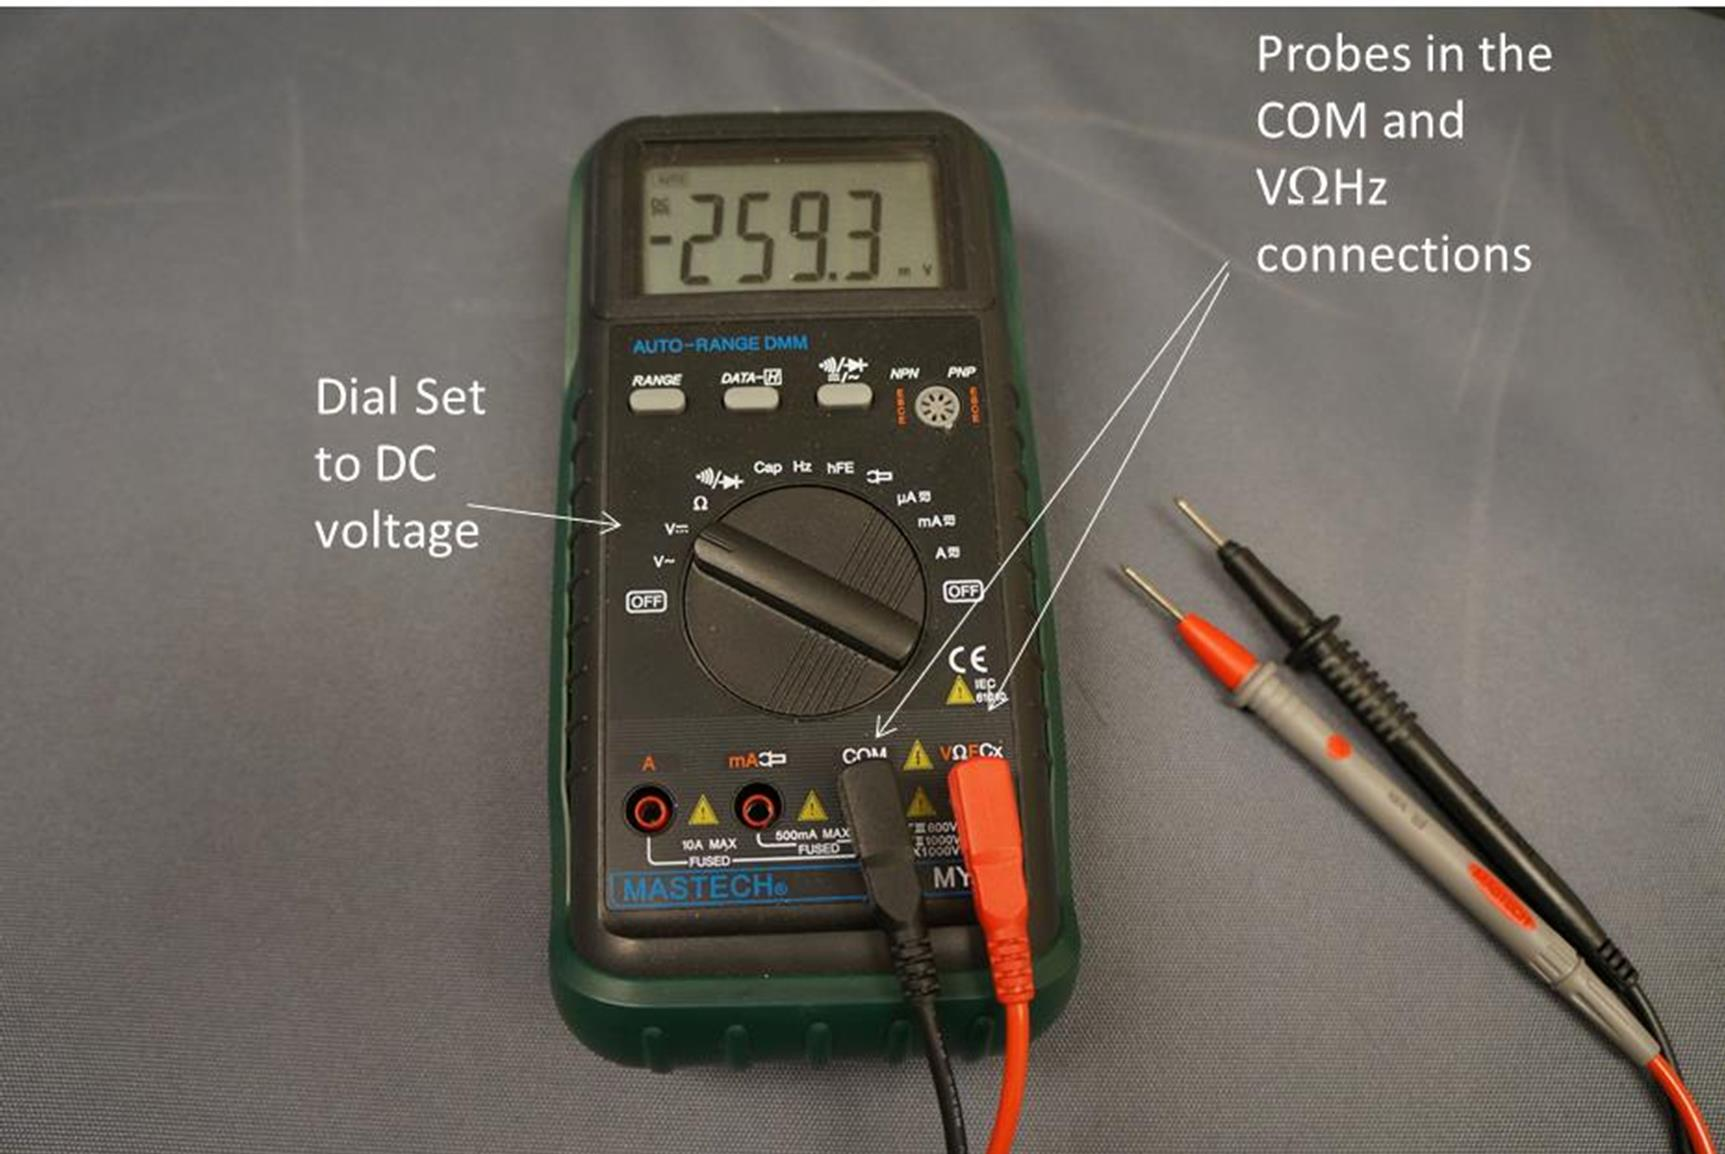
\includegraphics[width=2.9199in,height=1.962in]{PH4CAU0M}
\end{figure}

\begin{figure}[h!]
	\caption{AstroAI multimeter \label{AstroAI}}
	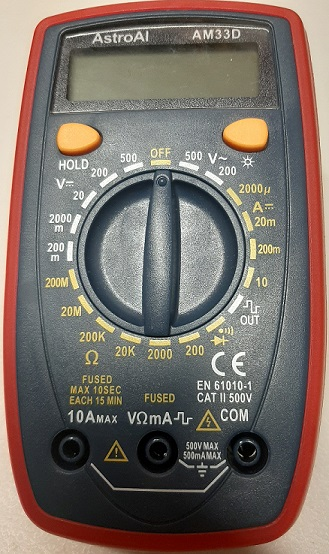
\includegraphics[width=2.5in]{AstroAIMultiMeter}
\end{figure}
\subsubsection{Signal Out}
You will notice that there are other settings besides volts. Our meters are all multi-meters. That means that they can measure more than one thing. We will use several of the settings throughout the semester. Take a look at the figure \ref{AstroAI} and also look at your own multimeter. One of the settings is unique to these multimeters.  It is white and can be found at about 4 o'clock on the dial. It has a square squiggle and simply says ``OUT''. This is an output signal like what you would see from a signal generator, see section \ref{siggen}. Only this is a fixed signal that oscillates at 50 times a second and goes from -5V to 5V. 

\subsubsection{Current}

Our multimeters have a current setting as well as a voltage setting. Current
is a flow of charge. This is like a water current, which is a flow of water.
Only we have a different thing flowing. We have a flow of charge. In the
wires in our Arduino, the moving charged things are (mostly) electrons. We
can write the flow of something as 
\begin{equation*}
I=\frac{\Delta Q}{\Delta t}
\end{equation*}%
where for us $\Delta Q$ is the amount of charge that has gone by in the time 
$\Delta t.$ Physicists use the letter $I$ for electrical current.

We should take a minute to think about what to expect when we allow charge
to flow. Think of a garden hose. If the hose is full of water, then when we
open the faucet, water immediately comes out. The water that leaves the
faucet is far from the open end of the hose, though. We have to wait for it
to travel the entire length of the hose. But we get water out of the hose
immediately! Why? \begin{figure}[h!]
	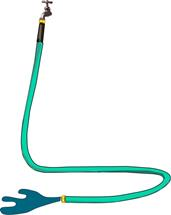
\includegraphics[width=1.4547in,height=1.8228in]{PH4CAU0V}
\end{figure}The new water coming in causes a
pressure change that is transmitted through the hose. The water at the open
end is pushed out. You can tell this is the case because the water
immediately leaving the hose is warm and tastes like plastic hose. After a
while, the water is colder and cleaner.

Current is a little bit like this. When we flip a light switch, the
electrons near the switch start to flow. But there are already free
electrons in the wire. These experience a push that makes the light turn on
almost instantly. But the electrons that turn on the light are not the ones
that just went through the switch.

\subsubsection{Measuring Current}
\label{MeasureA}
Because current is a flow, to measure current we must put a meter into that
flow. In a house, if you want to measure how much water is used, you connect
the pipe from the city water system to a meter. The water flows through the
meter and then goes into the pipe that brings water to the house. That way,
the meter can't miss any of the water (and the city can't miss any of your
payment!). The same is true for electrical current. To measure electrical
current, we need to remove part of our circuit, and replace it with the
meter to force the flow of electrical current to go through the meter. A
schematic diagram of this might look like this: \begin{figure}[h!]
	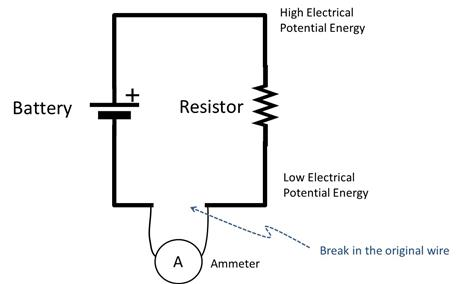
\includegraphics[width=3.8484in,height=%
	2.3981in]{PH4CAU0W}
\end{figure}In this diagram, you can see that
the electric current must go through the current meter. In fact, it couldn't
go anywhere else because part of the original circuit wire is missing. This
is just what we want. To actually perform this measurement with one of our
multimeters you could set up a circuit like the one in the following figure. 
\begin{figure}[h!]
	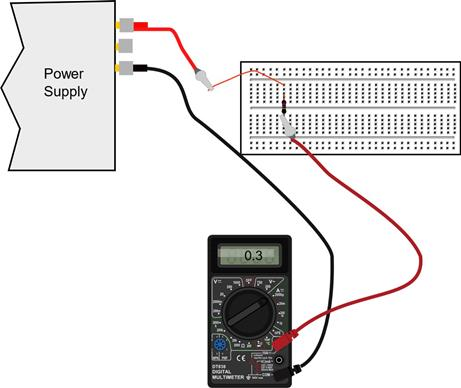
\includegraphics[width=3.8821in,height=3.2707in]{PH4CAU0X}
\end{figure}There is one more important thing
to do to make this work. We need to change the meter settings. And there are
two separate changes. The first is to switch the probe connections. One
probe stays in the COM or common connector, but the other needs to move to
the connector marked with an \textquotedblleft A.\textquotedblright\ Here is
an example showing the changes with two kinds of multimeters. \begin{figure}[h!]
	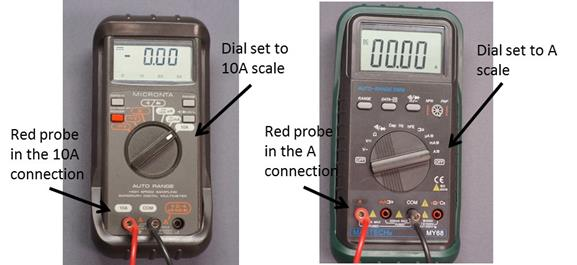
\includegraphics[width=%
	4.858in,height=2.2423in]{PH4CAU0Y}
\end{figure}The \textquotedblleft
A\textquotedblright\ stands for the standard unit of electrical current, the
Ampere or Amp. With the multimeter set up like this we would call it an 
\emph{ammeter}. Ammeters measure electrical current.



\subsection{Arduino as Power Supply and Voltmeter}
\label{ArduinoTour}
The Arduino is a little mini computer that can also measure voltage. It also has a power supply for limited electronics. Take a look at your Arduino and compare it to figure \ref{ArduinoLayOut}.
\begin{figure}[h!]
	\caption{Arduino lay out\label{ArduinoLayOut}}
	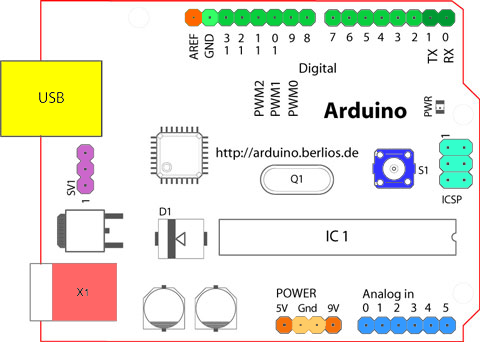
\includegraphics[width=3.116in]{arduino_board}
\end{figure}
Notice there are 3 main sets of pins (holes that you can put wires in). There are the digital pins, these are green in the figure. You used these last week to turn on and off a light. The blue ones are labeled Analog in. These are the same as a volt meter. Then there is the orange. These are kind of everything else. But we care most about the ones that are labeled with a V and Grd. These are voltage out and ground. 

The pins labeled 5V and 3.3V volts can be treated like a power supply. See section \ref{power}. But there are significant differences. The Arduino power pins can only output a single voltage, 3.3 or 5V. In addition they are very limited as to the amount of current they can supply at those voltages. They can only supply about 50mA. This is 60 times less than the desktop power supply described in a later section. 50mA is only enough to power a few LEDs. This will limit what we can do, but we should still be able to understand the physics. If you want to have more current you will need to get a different power supply. This could be as simple as a 9V battery, or maybe a plug in transformer from another device. This could come in useful when you are working on your student designed lab. For the other labs the 5V 50mA will be enough. 

The Analog in pins are also a lot like a voltmeter. But here again there are limitations. Thankfully there are also some really nice advantages as well. First the limitations. These pins can only measure voltages between 0V and 5V. The hand held voltmeter can go all the way from -500V to +500V. Also the analog pins can only measure to a certain precision. They can measure changes in voltage as small as about 4.9mV. This is significantly larger than the voltmeter.  Now for the good. Because these pins are attached to a mini computer the voltage can be measured over and over again. As often as about 10,000 times each second. Also we will see in later labs that these values can then be stored on a SD card to look at later. You can't do that with the hand held voltmeter! This is instead similar to a stand alone oscilloscope, see section \ref{oscilly}


\subsection{Power Supply}
\label{power}
A power supply is like an adjustable battery. Batteries have fixed voltages.
But a power supply may have an adjustable voltage. \begin{figure}[h!]
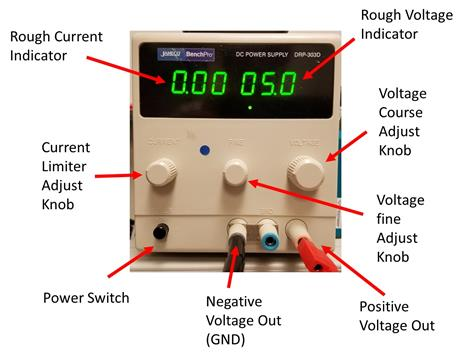
\includegraphics[width=3.9237in,height=%
3.0191in]{PH4CAU0I}
\end{figure}Usually a power supply takes
electrical energy from the wall outlets and converts that energy into the
specific voltage range that we want for our experiment. So it is like a
battery, but must be plugged into the wall. Our power supplies are designed
to keep us safe. They are current limited, meaning that they try not to give
too much charge flowing through our wires. Sometimes this is a problem
because they are too limited. There is a current limiting knob that you can
turn to allow a little more current. Be careful when you use this. The
voltage may jump wildly when you turn the current knob! It is best to turn
all the knobs down as low as they will go before you turn on the power
supply. Then, after turning on the power supply, increase the current knob
about half a turn and then slowly turn the voltage knob up to your desired
voltage. If the voltage stops increasing, turn the voltage knob back down a
bit, and turn up your current limiter knob some more. Then try your voltage
knob again.

Some of our electrical devices are quite delicate, and will literally burn
up if you apply too much current or voltage. In today's lab, we will
practice using our power supply so we are prepared when the delicate
components come out later.

\subsection{Signal Generator}
\label{siggen}
\begin{figure}[h!]
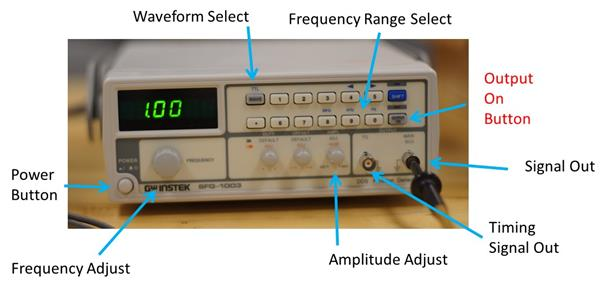
\includegraphics[width=5.093in,height=2.4348in]{PH4CAU0J}
\end{figure}The signal generator is a fancy
power supply. It makes changing voltages. It can make voltages in sine,
square, and triangle patterns. These time-varying signals have a maximum
voltage (called the amplitude) . We will use both the wave output and a
timing signal that the wave generator creates. Each has their own Bayonet
Neill--Concelman connector (usually just called a BNC connector) on the
front of the signal generator. You will need a cable with BNC connectors on
one end (and maybe alligator clips on the other end) to use this device.
There is an amplitude knob on the front of the signal generator. Because the
signal generator makes a voltage that changes in time, the amplitude of the
signal must be in voltage units. We should be careful not to set the signal
amplitude (voltage) too high or we run the risk of destroying our measuring
devices. Again turn the amplitude (voltage) down before you connect the box
to our electrical components. Then turn up the voltage to what you want in a
safe way.

There are frequency range buttons (using the shift button) near the middle
of the device panel. To change the frequency, you use the shift and range
buttons to set which digit you are adjusting, then turn the frequency knob
to make the change. An annoying feature of our frequency generators is that
you must push the \textquotedblleft output on\textquotedblright\ button or
they don't output a signal. When everything is set up right, we get a sine
wave (or square wave, or triangle wave) out. Here is a signal from the
signal generator displayed on one of our measuring devices, the
oscilloscope. \begin{figure}[h!]
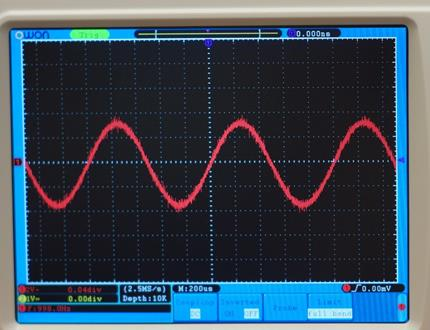
\includegraphics[width=3.6262in,height=2.7882in]{PH4CAU0K}
\end{figure}

Of course, simple batteries are sources of voltage, and so are many other
things.



\subsection{Oscilloscope}
\label{oscilly}
Our next device, the oscilloscope, is just a fancy voltmeter. Unlike the
multimeter, it usually just measures voltage. But it does it with flare!

The oscilloscope can measure changing voltages very accurately and usually
has a way to graph the changing voltage. The standard is a voltage vs. time
graph. A sinusoidally varying voltage should look something like this when
plotted. \begin{figure}[h!]
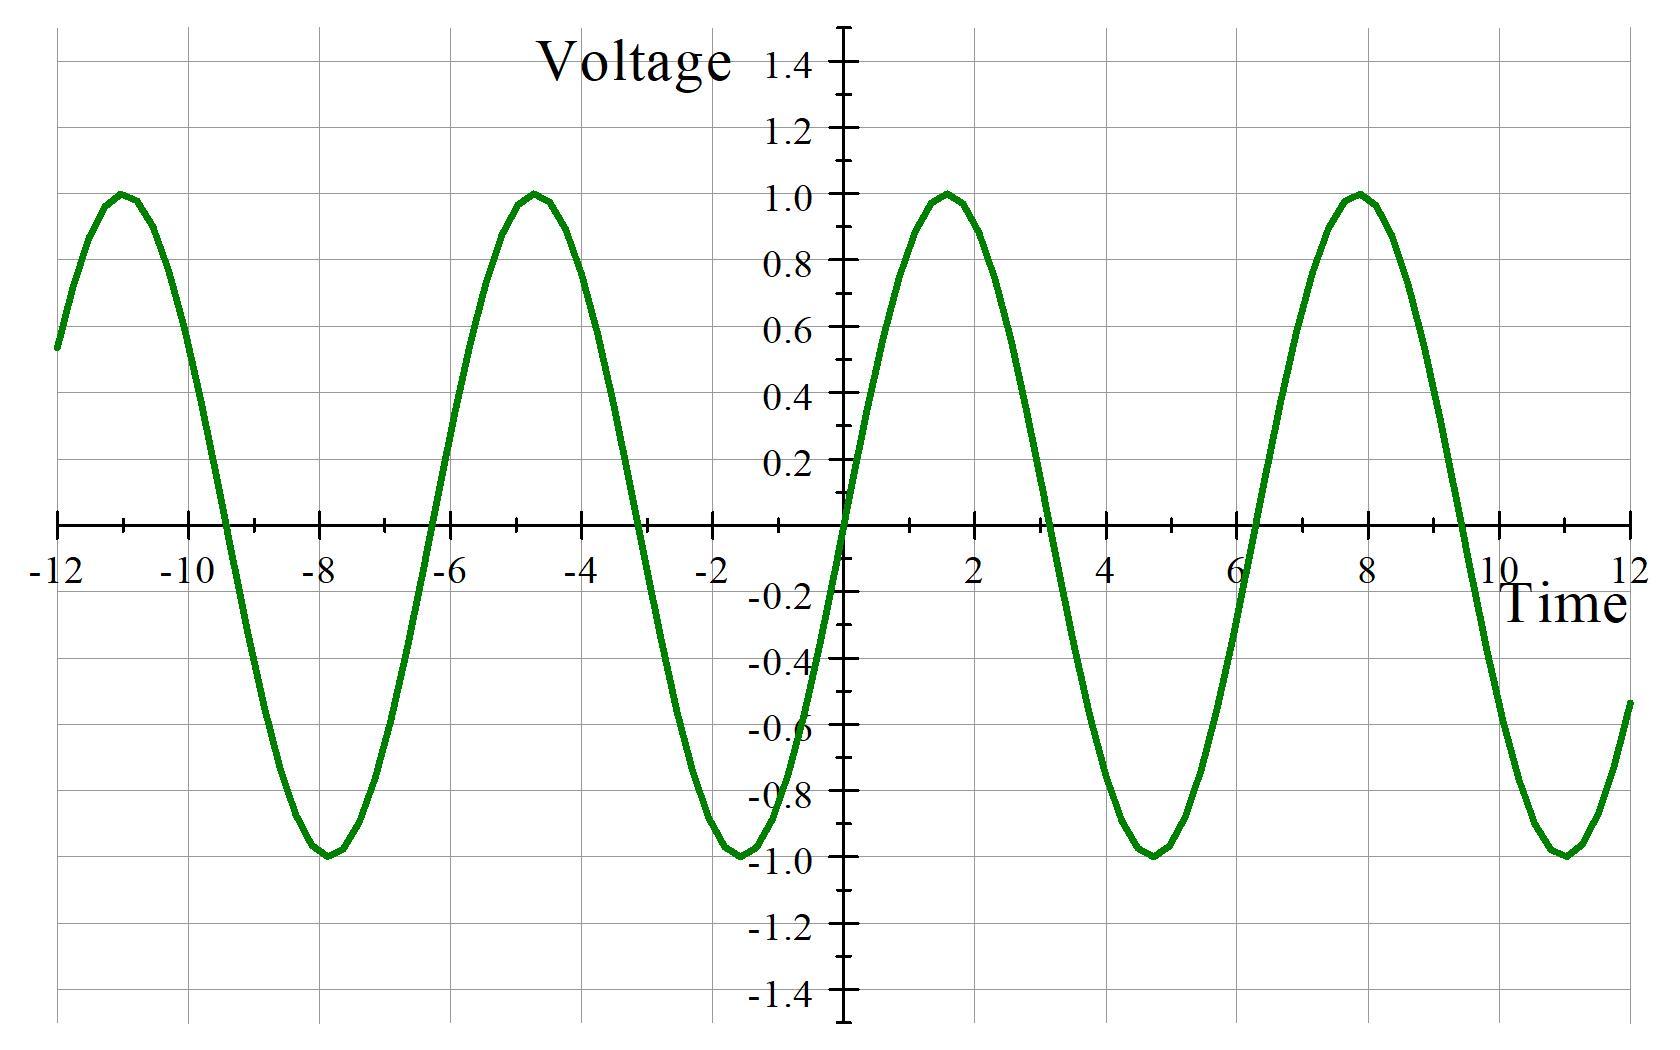
\includegraphics[width=4.4997in,height=3.0007in]{PH4CAU0N}
\end{figure}And that is what our oscilloscope
does. We should see something like this on the oscilloscope screen. From our
discussion of the signal generator, you know that this is just what we see.%
\begin{figure}[h!]
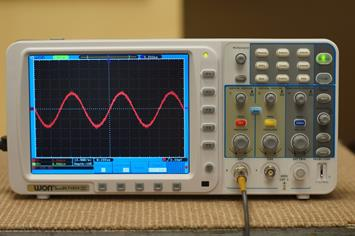
\includegraphics[width=2.998in,height=1.9993in]{PH4CAU0O}
\end{figure}

If the changing voltage is periodic, the oscilloscope has a way to use this
fact to stabilize the graph so you can see the details more clearly. This
stabilization is called \textquotedblleft triggering\textquotedblright\ and
on our oscilloscopes there are buttons and knobs on the right hand side of
the oscilloscope that adjust the triggering to make the graph more stable
(or less stable). The photograph of the sine wave above was taken by
stabilizing a sine wave from our signal generator. The oscilloscope starts
plotting at the same part of the wave each time, so the periodic signal
seems to stand still. To do this we must \textquotedblleft
trigger\textquotedblright\ the graph at some good starting point. Our
oscilloscopes have a build-in circuit that can watch for the same part of a
signal and start the graph in the same place each time. One of the knobs
adjusts the trigger point. \begin{figure}[h!]
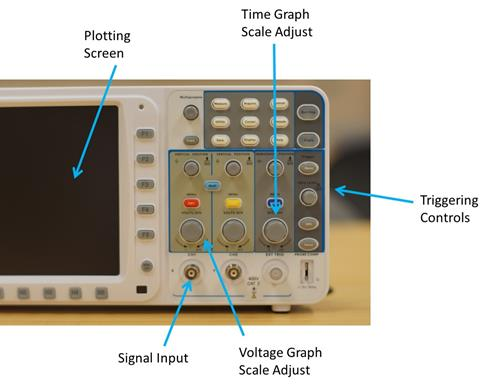
\includegraphics[width=4.23in,height=3.2659in]{PH4CAU0P}
\end{figure}The other controls adjust the
horizontal and vertical axes. The vertical axis is voltage, and the voltage
axis control is next to the signal input toward the bottom middle of the
front panel. To the right of this is the horizontal axis control, which is
time. You can choose how many volts per division with one knob and how many
seconds (or fractions of seconds) per division you have on your graph with
another knob. In the next figure you can see a signal on the oscilloscope
screen. \begin{figure}[h!]
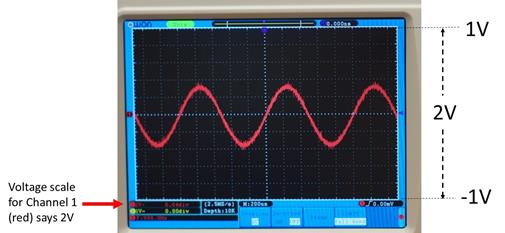
\includegraphics[width=4.2505in,height=1.9718in]{PH4CAU0Q}
\end{figure}In the bottom left-hand corner
there is a red dot and a voltage given. This is the voltage displayed across
the whole screen. Since when this photo was take the voltage knob was set to 
$2\unit{V}$, this means that the bottom of the screen represents $-1\unit{V}$
and the top of the screen represents $+1\unit{V}.$ \begin{figure}[h!]
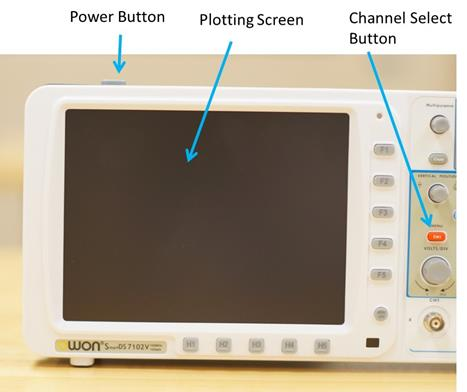
\includegraphics[width=3.9364in,height=%
3.3076in]{PH4CAU0R}
\end{figure}

There are two signal inputs because our oscilloscopes can look at two
different voltage signals at the same time. Each signal input is called a
\textquotedblleft channel.\textquotedblright\ Each channel has it's own
voltage scale knob and voltage scale indicator in the bottom left-hand
corner. They share the same time scale.

The channel inputs each have a BNC connector. We use oscilloscope probes
connected to these connectors. Notice that since there are two channels, an
oscilloscope can measure two voltages at once. But that means we may need
two probes!

To check that our oscilloscope is working correctly we can measure a known
voltage, say, the voltage of a regular battery.

\begin{figure}[h!]
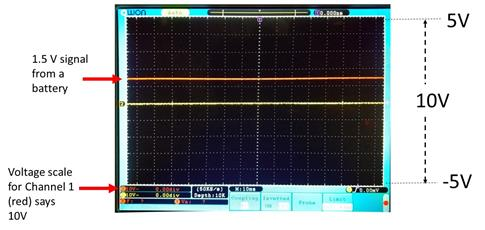
\includegraphics[width=4.0836in,height=1.9458in]{PH4CAU0S}
\end{figure}Notice that I changed the voltage
scale knob position so that now the oscilloscope screen has a $10\unit{V}$
total potential change. That means that we have $5\unit{V}$ at the top of
the screen and $-5\unit{V}$ at the bottom of the screen. The screen is
divided into little boxes. There are five rows of boxes from the bottom to
the top of the screen. Each box represents $1/10$ of the total voltage.
Since we have $\Delta V=10\unit{V},$ each box represents $\Delta V=1\unit{V}%
. $ So our battery voltage should give us one and a half boxes. And that is
just what we got.

But sometimes the oscilloscope does not get the right voltage. If this
happens we need to calibrate the oscilloscope. Every time we use an
Oscilloscope it is a good idea to check it to make sure it working well. Our
oscilloscopes have a test voltage to use just for this purpose.

\begin{figure}[h!]
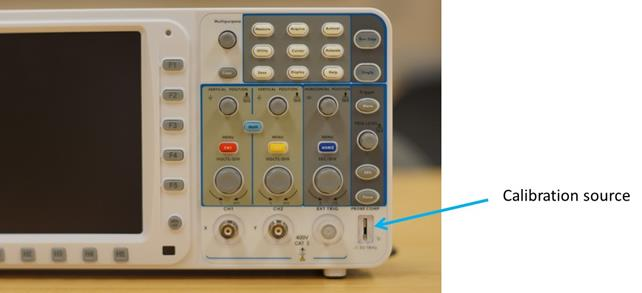
\includegraphics[width=5.3982in,height=2.4742in]{PH4CAU0T}
\end{figure}

The calibration source makes a $5\unit{V}$ square wave (try it to see what
that looks like!). If we use this calibration source we should get something
like what you see in the next figure. \begin{figure}[h!]
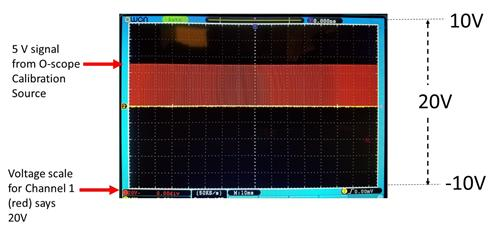
\includegraphics[width=4.2004in,height=1.9623in]{PH4CAU0U}
\end{figure}If you don't get $5\unit{V},$
then some thing is wrong and you will need to go through the oscilloscope's
calibration procedure. That is in the oscilloscope manual and you can find
the manual on-line.








\section{Lab Assignment}


%\subsection{Practice Measurements}

\subsection{Use a Multimeter}

\begin{enumerate}
	\item Measure the voltage of a 9-V battery with a voltmeter. Report the
	value you get from the measurement and the uncertainty.
	
	\item Set up the circuit described in section (\ref{Voltage Measurement with
		Meter}). The figure is repeated below. Measure the voltage with a
	multimeter. Use the Arduino 5V power supply and ground. Do you measure exactly 5V?
	\begin{figure}[h!]
		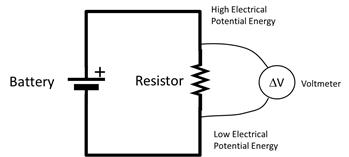
\includegraphics[width=2.9438in,height=1.3353in]{PH4CAU1G}
	\end{figure}
	
	\item Modify your circuit to measure current as described in section (\ref{MeasureA}) and change the settings of your multimeter so that you measure the current in the circuit. Connecting the multimeter probes can be problematic in this situation because the connections themselves can act like resistors. Don't worry to much about this during this lab. We will explore this issue more in the next lab. For now I just want you to get experience using the multimeter to measure current. 
\end{enumerate}


\subsection{Simple Arduino Voltmeter}

\begin{enumerate}
	\item Put the circuit back together to measure voltage again.
	 \begin{figure}[h!]
		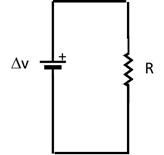
\includegraphics[width=1.3932in,height=1.3188in]{PH4CAU1Z}
	\end{figure}(see section (\ref{Voltage
		Measurement with Meter}). \begin{figure}[h!]
		
\includegraphics[width=1.8507in,height=0.9677in]{PH4CAU20}
	\end{figure}This time write the simple voltmeter sketch, wire it up, and measure the voltage across the resistor
	using our Arduino and the serial monitor. Be careful trying to measure any voltage out side the $0$ to $5\unit{V}$ range could damage your Arduino!
	
	%\item Calculate the uncertainty due to quantization error for your Arduino	simple voltmeter
	
	%\item Compare your calculated uncertainty to the measured uncertainty that you see in your device output. (This is tricky, does the power supply give a truly constant voltage?)


\end{enumerate}












\subsection{Seeing the data}

Once the code is compiled and uploaded, the Arduino will send data to the
serial port. The serial monitor can display the data. The serial monitor is
found under the Arduino Software Tools menu. See figure \ref{tools}

\begin{figure}[h!]
	\caption{Arduino IDE Tools\label{tools}}
	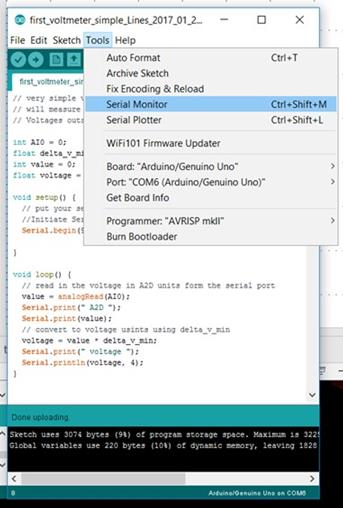
\includegraphics[width=2.0807in,height=3.0744in]{PH4CAU1P}
\end{figure}
You should then see something like figure \ref{monitor}

\begin{figure}[h!]
	\caption{Arduino Serial Monitor\label{monitor}}
	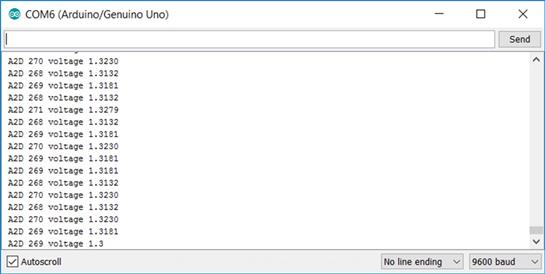
\includegraphics[width=4.5861in,height=2.3151in]{PH4CAU1Q}
\end{figure}

The Arduino Software can also plot the data from the serial port. Here is a
plot of the same data that we saw on the serial monitor. 
\begin{figure}[h!]
	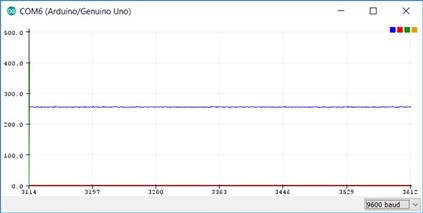
\includegraphics[width=%
	3.563in,height=1.8049in]{PH4CAU1R}
\end{figure}
Notice that it plotted our voltage values and it also plotted our ADC values. This makes the voltage
values hard to see. We could fix this by commenting out the lines that print
the ADC values (putting \textquotedblleft //\textquotedblright\ at the
beginning of the line). Then those lines won't be executed by the Arduino.
Then we get just the voltage. 
\begin{figure}[h!]
	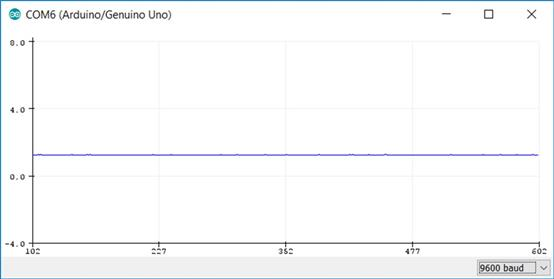
\includegraphics[width=3.2578in,height=1.6475in]{PH4CAU1S}
\end{figure}
Notice that the horizontal axis
is not exactly time. It is just the data point number. We could convert this
to time with some calculation if we know how often the Arduino sends us a
data point. I will leave this as an exercise.




\subsection{Measuring a Changing Voltage}
Using the same code measure the voltage from the "OUT" on your AstroAI multimeter. In other words conect the probes from the multimeter to the ground and one of the Analog in pins on the Arduino. Be sure the multimeter dial is set to the "OUT" position. Then run the voltage measuring code on your Arduino. This time instead of opening the "Serial Monitor" try looking at the "Serial Plotter".  What do you see? Try changing the amount of time the program waits between loops. This is done by adding the commend "delay(3)". The 3 is the amount of milliseconds that the Arduino will wait before continuing on with the loop. Change the time. Try 10, 20, 21, 40, and others. How does that affect what you see and why? Remember the voltage signal from the multimeter is -5$\unit{V}$ to +5$\unit{V}$ that cycles 50 times every second (50$\unit{Hz}$).



	
	
	
	
\subsection{Voltage Divider}
	
	\begin{enumerate}
		\item Build the voltage divider using two resistors as shown in figure \ref{VoltageDivider}. You will have to think about which resistors from our set will work best. Discuss this with your group, or have group members try the calculations with different combinations. Use the 5$\unit{V}$ power from the Arduino for your power supply
		\begin{figure}[h!]
			\caption{Voltage Divider\label{VoltageDivider}}
			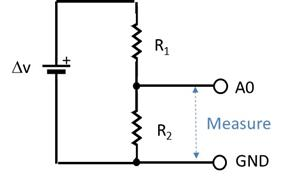
\includegraphics[width=2.3851in,height=1.5469in]{PH4CAU22}
		\end{figure}
		
		\item Use a multimeter to verify that the output of the voltage divider (the voltage between the resistors) is at least roughly what you would expect.  Try switching the power voltage to the 3.3$\unit{V}$ and check again with the multimeter what the voltage is between the resistors.
		
%		\item \begin{figure}[h!]
%			
\includegraphics[width=1.8507in,height=0.9677in]{PH4CAU21}
%		\end{figure}
		
		\item Write the sketch (the code) and then hook the output of your voltage divider to the A0 pin and the other side of $ R_{2} $ to a GND pin.

		Your Arduino voltmeter should now be set up. Compile and load the sketch and use the Serial Plotter to watch the voltage values as you change the power supply from $5$ to $3.3\unit{V}$. 
		
		%\item What is the quantization error for this voltmeter? Check to see if this matches your values on the serial monitor.
		
		%\item Design a voltage divider that will allow the full $0$ to $30\unit{V}$ range of our power supply to be measured using the Arduino's $0$ to $5\unit{V}$ analog input. What would the quantization error be for this new circuit?
		
		\item The analog in pins can only measure voltages less than 5$\unit{V}$ and greater than 0$\unit{V}$. Can you think of a way you could measure voltages higher than 5$\unit{V}$ with the Arduino?
		
	\end{enumerate}






%TCIMACRO{\TeXButton{\vspace*{\fill}}{\vspace*{\fill}}}%
%BeginExpansion
\vspace*{\fill}%
%EndExpansion
\pagebreak


%\section{Extending our voltmeter with a voltage divider\label{Voltmeter with
%		Voltage Divider}}
%
%This Arduino-based voltmeter that we have built is great, but will only let
%us measure voltages in the range $0$ to $5\unit{V}.$ That seems a little
%restrictive. We would like to extend our voltmeter to a larger range, say, $%
%0 $ to $20\unit{V}.$ To do this, we will need to add some electronic
%components and think about what we have learned about voltage, resistance,
%and current. Let's consider this circuit.\begin{figure}[h!]
%	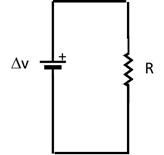
\includegraphics[width=1.3932in,height=1.3188in]{PH4CAU1T}
%\end{figure}We have a battery, That will make
%the current flow much like a pump makes water move through pipes.
%
%\begin{figure}[h!]
%	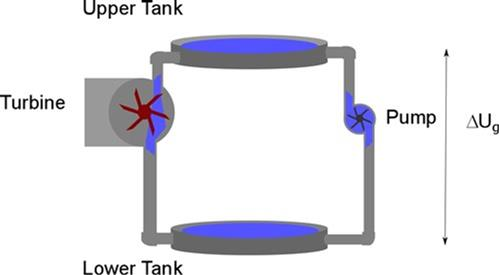
\includegraphics[width=4.2004in,height=2.3229in]{PH4CAU1U}
%\end{figure}The water in a pipe system gains
%potential energy as it moves up. In our circuit we will find that electric
%charge gains potential energy as we move it across a battery. Then the
%charge will move down the wire like water moves down a pipe until it is out
%of potential energy. Notice that the water in a pipe system will lose all
%the potential energy that it gained when the pump raised it to the upper
%tank (see previous figure). That is true of electric charge too. The
%electric current travels from the battery through the resistor, but in doing
%so it loses all the potential energy that the battery gave it by the time it
%returns to the battery.
%
%Now suppose we have two resistors in a circuit. \begin{figure}[h!]
%	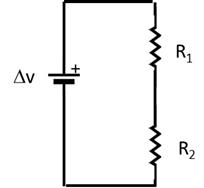
\includegraphics[width=1.7279in,height=%
%	1.5947in]{PH4CAU1V}
%\end{figure}
%
%Our water analogy can still help us understand what will happen. Suppose
%that we have two turbines in our pipe system. \begin{figure}[h!]
%	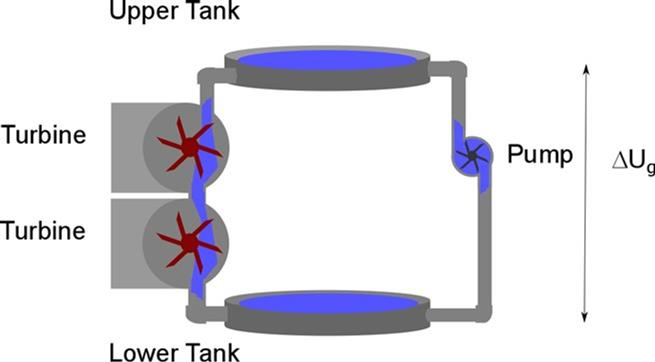
\includegraphics[width=3.5985in,height=%
%	1.9934in]{PH4CAU1W}
%\end{figure}The water leaves the high
%potential energy part of the pump, and is put to work turning the first
%turbine. The resistance of the turbine will slow the water current. So when
%the water leaves the turbine, it will have lost some potential energy. Since
%we have a second turbine the current will again be slowed and more potential
%energy will be lost. How much potential energy do we lose as the water
%falls? All of the potential energy that the pump gave it! We must end up
%with the water at the bottom back at the low potential energy. We will find
%this to be true for our electric circuit as well. We will loose some
%potential energy as the electrical energy \textquotedblleft
%falls\textquotedblright\ from the high electric potential \textquotedblleft
%down\textquotedblright\ the first resistor. After the second resistor, we
%can guess that we must be back at the low electric potential we started with.
%
%\begin{figure}[h!]
%	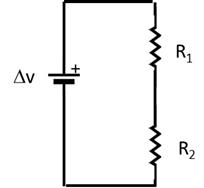
\includegraphics[width=1.7279in,height=1.5947in]{PH4CAU1X}
%\end{figure}We know that electric potential
%is a potential energy per unit charge. And energies just add up. If 
%\begin{equation*}
%\Delta V=RI
%\end{equation*}%
%is satisfied, then we would expect that adding two resistors would just
%linearly add the effects of the two resistors together%
%\begin{eqnarray*}
%	\Delta V_{total} &=&\Delta V_{1}+\Delta V_{2} \\
%	&=&R_{1}I+R_{2}I
%\end{eqnarray*}%
%Note that the same current must flow through each of the resistors, since
%the current leaving $R_{1}$ is the current flowing into $R_{2}.$ Then 
%\begin{equation*}
%\Delta V_{total}=\left( R_{1}+R_{2}\right) I
%\end{equation*}%
%Our current will be 
%\begin{equation*}
%I=\frac{\Delta V_{total}}{R_{1}+R_{2}}
%\end{equation*}
%
%But suppose we measure the potential change across just resistor $R_{2}.$ 
%\begin{figure}[h!]
%	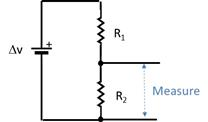
\includegraphics[width=1.7625in,height=1.0421in]{PH4CAU1Y}
%\end{figure}what would we expect to get? We
%lost voltage across both $\Delta V_{1}$ and $\Delta V_{2}$ so 
%\begin{equation*}
%\Delta V_{total}=\Delta V_{1}+\Delta V_{2}
%\end{equation*}%
%because we must loose all the $\Delta V_{total}$ given to the current by the
%battery. And 
%\begin{equation*}
%\Delta V_{2}=IR_{2}
%\end{equation*}%
%from Ohm's law. So
%
%\begin{equation*}
%\Delta V_{2}=\left( \frac{\Delta V_{total}}{R_{1}+R_{2}}\right) R_{2}
%\end{equation*}%
%This is only part of the total voltage. And if we have two different
%resistors so that $R_{1}\neq R_{2}$ then we can choose for $\Delta V_{2}$ to
%be nearly as much as $\Delta V_{total}$ or nearly as little as $0$ by
%carefully choosing our two resistances. We call a set of two resistors like
%this a \textquotedblleft voltage divider\textquotedblright\ because it
%divides the battery voltage between the two resistors. If $R_{1}$ is bigger
%than $R_{2}$ then $\Delta V_{1}$ is bigger than $\Delta V_{2}.$
%
%Remember that the input can only withstand $0$ to $5\unit{V}.$ More than
%that can destroy the board! But we want to measure a voltage that varies
%from $0$ to $20\unit{V}.$ We now have a way to do this. We will use a
%voltage divider. The voltage across both resistors will be as much as $20%
%\unit{V},$ but we will measure the voltage across only one of the resistors.
%And we will choose our resistor so that when the total voltage is $20\unit{V}
%$ but the voltage across our resistor is $5\unit{V}$ (or less). Since we
%will know the resistances, we can use a little math to calculate what the
%total voltage was using the voltage measurement from just one of the
%resistors.
%
%This is like what we did to measure current last lab. We used a voltmeter
%and a resistor and some math to make an ammeter. Today we will use two
%resistors, our Arduino voltmeter, and some math to make a new voltmeter that
%can measure higher voltages. We just need to choose our resistors so that we
%map our $0$ to $20\unit{V}$ to $0$ to $5\unit{V}.$ Once choice might be 
%\begin{eqnarray*}
%	R_{1} &=&40\unit{k%
%		%TCIMACRO{\U{3a9}}%
%		%BeginExpansion
%		\Omega%
%		%EndExpansion
%	} \\
%	R_{2} &=&10\unit{k%
%		%TCIMACRO{\U{3a9}}%
%		%BeginExpansion
%		\Omega%
%		%EndExpansion
%	}
%\end{eqnarray*}%
%Let's try it. We would get%
%\begin{eqnarray*}
%	\Delta V_{2\max } &=&\left( \frac{20\unit{V}}{40\unit{k%
%			%TCIMACRO{\U{3a9}}%
%			%BeginExpansion
%			\Omega%
%			%EndExpansion
%		}+10\unit{k%
%			%TCIMACRO{\U{3a9}}%
%			%BeginExpansion
%			\Omega%
%			%EndExpansion
%	}}\right) \left( 10\unit{k%
%		%TCIMACRO{\U{3a9}}%
%		%BeginExpansion
%		\Omega%
%		%EndExpansion
%	}\right) \\
%	&=&4.0\unit{V}
%\end{eqnarray*}%
%when $\Delta V_{total}=20\unit{V}$ and 
%\begin{eqnarray*}
%	\Delta V_{2\min } &=&\left( \frac{0\unit{V}}{40\unit{k%
%			%TCIMACRO{\U{3a9}}%
%			%BeginExpansion
%			\Omega%
%			%EndExpansion
%		}+10\unit{k%
%			%TCIMACRO{\U{3a9}}%
%			%BeginExpansion
%			\Omega%
%			%EndExpansion
%	}}\right) \left( 10\unit{k%
%		%TCIMACRO{\U{3a9}}%
%		%BeginExpansion
%		\Omega%
%		%EndExpansion
%	}\right) \\
%	&=&0\unit{V}
%\end{eqnarray*}%
%when $\Delta V_{total}=0\unit{V}.$ Notice that this really didn't work. We
%only got a maximum voltage of $4\unit{V}.$ But this gives us a margin of
%safety. If we give our Arduino more than $5\unit{V}$ we can burn it up. If
%we plan our circuit so we don't get to close to $5\unit{V}$ we are safer. So
%this set of resisters is not a terrible choice.
%
%To report out our voltage we need to do this conversion backwards. Say we
%have $\Delta V_{total}=10\unit{V}$ that we are measuring with our new
%instrument. Then 
%\begin{eqnarray*}
%	\Delta V_{2} &=&\left( \frac{10\unit{V}}{40\unit{k%
%			%TCIMACRO{\U{3a9}}%
%			%BeginExpansion
%			\Omega%
%			%EndExpansion
%		}+10\unit{k%
%			%TCIMACRO{\U{3a9}}%
%			%BeginExpansion
%			\Omega%
%			%EndExpansion
%	}}\right) \left( 10\unit{k%
%		%TCIMACRO{\U{3a9}}%
%		%BeginExpansion
%		\Omega%
%		%EndExpansion
%	}\right) \\
%	&=&2\unit{V}
%\end{eqnarray*}
%
%The $2\unit{V}$ is what we actually measure at the A0 input. But we know
%that this represents $10\unit{V}$ across both resistors, so we want the
%Arduino program to print out $10\unit{V}.$ So we report%
%\begin{equation*}
%\Delta V_{reported}=\frac{\Delta V_{2}}{R_{2}}\left( R_{1}+R_{2}\right)
%\end{equation*}%
%or for our case, since we measured $2\unit{V}$ across our resistor,%
%\begin{equation*}
%10\unit{V}=\frac{2\unit{V}}{\left( 10\unit{k%
%		%TCIMACRO{\U{3a9}}%
%		%BeginExpansion
%		\Omega%
%		%EndExpansion
%	}\right) }\left( 40\unit{k%
%	%TCIMACRO{\U{3a9}}%
%	%BeginExpansion
%	\Omega%
%	%EndExpansion
%}+10\unit{k%
%	%TCIMACRO{\U{3a9}}%
%	%BeginExpansion
%	\Omega%
%	%EndExpansion
%}\right)
%\end{equation*}%
%We will have to write this math in our code. There is a further
%complication. The Arduino A0 input is giving us a number that represents $0$
%to $4\unit{V}$ for our setup. But that is not what we see on the serial
%port. We see a number from 0 to 1024. We know the $1024$ represents $5\unit{V%
%}$ and the $0$ represents $0\unit{V}.$ So we need to multiply the number
%that comes from our Arduino by $\delta V=4.9\unit{mV}$ once again to get our
%Arduino output into voltage units. So our reported voltage equation is
%something like this. 
%\begin{equation*}
%\Delta V_{reported}=A2D\times \delta V_{2}\times \frac{1}{R_{2}}\left(
%R_{1}+R_{2}\right)
%\end{equation*}
%
%All this calculation to get our reported voltage must do something to our
%measurement uncertainty. We could do our usual math to find the reported
%uncertainty, but instead, let's think. Every small voltage $\Delta V_{2}$
%would be multiplied by $\left( \frac{1}{R_{2}}\left( R_{1}+R_{2}\right)
%\right) $ to map it into our original $0\unit{V}$ to $20\unit{V}$ range.
%That should work for our smallest voltage that we can detect, namely $\delta
%V=4.9\unit{mV}.$ That is the smallest value $\Delta V_{2}$ could have. So in
%our $0\unit{V}$ to $20\unit{V}$ range the smallest value this can map to is 
%\begin{equation*}
%\delta V_{reported}=\left( \delta V\right) \left( \frac{1}{R_{2}}\left(
%R_{1}+R_{2}\right) \right)
%\end{equation*}%
%The first term in parenthesis is essentially $1$ digitizer unit multiplied
%by $\Delta V_{2}$ and the second term in parenthesis converts the $\Delta
%V_{2}$ value into actual volts measured across both resistors.
%
%The quantity $\delta V_{reported}$ gives us our quantization error value for
%our new instrument. Our output will be in multiples of 
%\begin{equation*}
%V_{reported}=n\times \delta V_{reported}
%\end{equation*}%
%Putting in numbers gives 
%\begin{eqnarray*}
%	\delta V_{reported} &=&\left( 4.\,\allowbreak 884\times 10^{-3}\unit{V}%
%	\right) \left( \frac{1}{10\unit{k%
%			%TCIMACRO{\U{3a9}}%
%			%BeginExpansion
%			\Omega%
%			%EndExpansion
%	}}\left( 40\unit{k%
%		%TCIMACRO{\U{3a9}}%
%		%BeginExpansion
%		\Omega%
%		%EndExpansion
%	}+10\unit{k%
%		%TCIMACRO{\U{3a9}}%
%		%BeginExpansion
%		\Omega%
%		%EndExpansion
%	}\right) \right) \\
%	&=&0.024\,42\unit{V} \\
%	&=&24.42\unit{mV}
%\end{eqnarray*}%
%This is much bigger than our $4.9\unit{mV}$ uncertainty for the simple
%voltmeter. And this is the cost of using a voltage divider to extend our
%voltage range. For the bigger voltage range we get a bigger uncertainty.
%
%Let's try another example. Suppose we wish to measure $0$ to $20\unit{V}$
%and we look in our case of resistors and find we have the following two
%resistors to use:%
%\begin{eqnarray*}
%	R_{1} &=&98\unit{k%
%		%TCIMACRO{\U{3a9}}%
%		%BeginExpansion
%		\Omega%
%		%EndExpansion
%	} \\
%	R_{2} &=&15\unit{k%
%		%TCIMACRO{\U{3a9}}%
%		%BeginExpansion
%		\Omega%
%		%EndExpansion
%	}
%\end{eqnarray*}
%
%We would expect that our $0$ to $20\unit{V}$ would be mapped to a smaller
%range. Let's find that range.%
%\begin{eqnarray*}
%	\Delta V_{2\max } &=&\left( \frac{20\unit{V}}{98\unit{k%
%			%TCIMACRO{\U{3a9}}%
%			%BeginExpansion
%			\Omega%
%			%EndExpansion
%		}+15\unit{k%
%			%TCIMACRO{\U{3a9}}%
%			%BeginExpansion
%			\Omega%
%			%EndExpansion
%	}}\right) \left( 15\unit{k%
%		%TCIMACRO{\U{3a9}}%
%		%BeginExpansion
%		\Omega%
%		%EndExpansion
%	}\right) \\
%	&=&2.\,\allowbreak 654\,9\unit{V}
%\end{eqnarray*}%
%So our voltage range at the Arduino A0 input will be $0\unit{V}$ to $%
%2.\,\allowbreak 65\unit{V}.$ This set of resistors won't use the full
%Arduino $0\unit{V}$ to $5\unit{V}$ range. But it will measure $0$ to $20%
%\unit{V}.$ The minimum detectable voltage for this new instrument design for
%our $0$ to $20\unit{V}$ source will be 
%\begin{eqnarray*}
%	\delta V_{reported} &=&\left( \delta V_{2}\right) \left( \frac{1}{R_{2}}%
%	\left( R_{1}+R_{2}\right) \right) \\
%	&=&\left( 4.\,\allowbreak 880\,3\times 10^{-3}\unit{V}\right) \left( \frac{1%
%	}{\left( 15\unit{k%
%			%TCIMACRO{\U{3a9}}%
%			%BeginExpansion
%			\Omega%
%			%EndExpansion
%		}\right) }\left( 98\unit{k%
%		%TCIMACRO{\U{3a9}}%
%		%BeginExpansion
%		\Omega%
%		%EndExpansion
%	}+15\unit{k%
%		%TCIMACRO{\U{3a9}}%
%		%BeginExpansion
%		\Omega%
%		%EndExpansion
%	}\right) \right) \\
%	&=&3.\,\allowbreak 676\,5\times 10^{-2}\unit{V} \\
%	&=&37\unit{mV}
%\end{eqnarray*}
%
%This uncertainty is much bigger than the uncertainty for our last choice of
%resistors. So $98\unit{k%
%	%TCIMACRO{\U{3a9}}%
%	%BeginExpansion
%	\Omega%
%	%EndExpansion
%}$ and $15\unit{k%
%	%TCIMACRO{\U{3a9}}%
%	%BeginExpansion
%	\Omega%
%	%EndExpansion
%}$ are not great choices even though they technically work.
%
%For your version of the voltmeter in lab, you will choose the resistor
%values to use. Here is an Arduino sketch to implement this extended volt
%meter. In it are the not-so-good $98\unit{k%
%	%TCIMACRO{\U{3a9}}%
%	%BeginExpansion
%	\Omega%
%	%EndExpansion
%}$ and $15\unit{k%
%	%TCIMACRO{\U{3a9}}%
%	%BeginExpansion
%	\Omega%
%	%EndExpansion
%},$ but of course \textbf{you should change the sketch to have your resistor
%	values}.
%\begin{lstlisting}[language=Arduino]
%/////////////////////////////////////////////////////////
%// Extended Voltmeter
%// This voltmeter with the values given below
%// is designed to measure a 0 to 20V range with 1024 
%// discrete values of with an uncertainty of about 0.02V
%/////////////////////////////////////////////////////////
%//set up a variable to represent Analog Input 0
%int AI0 = 0;         
%// Resistance of R1(put in your actual value here)
%float R1 = 98000.0; 
%// Resistance of R2(put in your actual value here)  
%float R2 = 15000.0;  
%
%int ADC_value = 0;    // Place to put the A2D values
%float voltage = 0.0;  // calculated signal voltage
%//mV Arduino's minimum detectable voltage
%float delta_v_min = 0.0049 
%
%/////////////////////////////////////////////////////////
%void setup() {
%//Initiate Serial Communication
%Serial.begin(9600);    //9600 baud rate
%}
%
%/////////////////////////////////////////////////////////
%void loop() {
%// read the serial data from AI0
%ADC_value = analogRead(AI0);
%// if you want to, print out the channel A2D values. 
%// Uncomment if you want them.
%//Serial.print("analog channel value ");
%//Serial.print(ADC_value);
%// calculate the signal voltage 
%voltage=ADC_value*(delta_v_min)*(R1+R2)/R2;
%// print out the signal voltage
%Serial.print(" voltage ");
%Serial.println(voltage, 4);  
%}
%/////////////////////////////////////////////////////////
%/////////////////////////////////////////////////////////
%\end{lstlisting}
%
%\bigskip Of course you will want to have another person check your math and
%wiring, and you should check your output voltage with a stand-alone meter
%before you plug into your Arduino.
%
%\section{Practice Problems}
%
%\rule{11cm}{0.03cm}
%
%Here is an example for you to work out on your own before class. Do this and
%compare your result to the results of the other people in your lab group as
%you come into class on lab day.
%
%Suppose we wish to measure $0$ to $15\unit{V}$ and we look in our case of
%resistors and find we have the following two resistors to use:%
%\begin{eqnarray*}
%	R_{1} &=&43.2\unit{k%
%		%TCIMACRO{\U{3a9}}%
%		%BeginExpansion
%		\Omega%
%		%EndExpansion
%	} \\
%	R_{2} &=&15.2\unit{k%
%		%TCIMACRO{\U{3a9}}%
%		%BeginExpansion
%		\Omega%
%		%EndExpansion
%	}
%\end{eqnarray*}%
%What range of voltages would we see at the Arduino, and what is the
%quantization error for our measurement?
%
%\rule{11cm}{0.03cm}
